\documentclass[
	10pt,								% globale Schriftgröße
	parskip=half-,						% setzt Absatzabstand hoch
	paper=a4,							% Format
	english,ngerman,					% lädt Sprachpakete
	]{scrartcl}							% Dokumentenklasse

% //////////////////// Pakete laden ////////////////////
\usepackage{amsmath}			% MUSS vor fontspec geladen werden
\usepackage{mathtools}			% modifiziert amsmath
\usepackage{amssymb}			% mathematische symbole, für \ceckmarks
\usepackage{amsthm}				% für proof
\usepackage{mathrsfs}			% für \mathscr
\usepackage{latexsym}
\usepackage{marvosym}				% für Lightning

\usepackage{fontspec} 			% funktioniert nur mit den neueren Compilern z.B. XeLaTeX
\usepackage{microtype}			% für bessere Worttrennung
\usepackage[ngerman]{babel} 	% Spracheinstellung
\usepackage{lmodern}			% verändert verwendete Schriftart, damit sie weniger pixelig ist

\usepackage{verbatim}
\usepackage{listings}			% Für Quellcode

\usepackage{graphicx}
\usepackage{tabularx}			% für Tabellen mit gleicher Spaltenbreite und automatischen Umbrüchen
\usepackage{fullpage}
\usepackage{multirow}			% für multirow in tabulars
\usepackage{rotate}
\usepackage[cmyk,table]{xcolor} % um Farben zu benutzen, kann mehr als das Paket color
\usepackage[					% Verlinkungen
	colorlinks,					% farbige Schrift, statt farbiger Rahmen
	linktocpage,				% verlinkt im Abb.Verzeichnis Seitenzahl statt Bildunterschrift
	linkcolor=blue				% setzt Farbe der Links auf blau
	]{hyperref}					% nur für digitale Anwendungen, url = "http://www.example.com"
\usepackage{url}				% für Webadressen wie e-mail usw.: "\url{http://www.example.com}"

\usepackage{enumerate}			% für versch. Aufzählungezeichen wie z.B. a)
\usepackage{xspace}				% folgt ein Leerzeichen nach einem \Befehl, wird es nicht verschluckt.
\usepackage{cancel}				% für das Durchstreichen u.a. in Matheformeln mit \cancel
\usepackage{float}              % zum Forcieren der Position von figure-Umgebungen

% zum Zeichnen (u.a. von Graphen)
\usepackage{fp}
\usepackage{tikz}
\usetikzlibrary{tikzmark}			% für \tikzmark{toRemember}
\usetikzlibrary{positioning}	% verbesserte Positionierung der Knoten
\usetikzlibrary{automata}		% für Automaten (GTI)
\usetikzlibrary{arrows}
\usetikzlibrary{shapes}
\usetikzlibrary{decorations.pathmorphing}
\usetikzlibrary{decorations.pathreplacing}
\usetikzlibrary{decorations.shapes}
\usetikzlibrary{decorations.text}

% //////////////////// Syntaxhighlighting ////////////////////
\lstloadlanguages{Python, Haskell, [LaTeX]TeX, Java}
\lstset{
   basicstyle=\footnotesize\ttfamily,	% \scriptsize the size of the fonts that are used for the code
   backgroundcolor = \color{bgcolour},	% legt Farbe der Box fest
   breakatwhitespace=false,	% sets if automatic breaks should only happen at whitespace
   breaklines=true,			% sets automatic line breaking
   captionpos=t,				% sets the caption-position to bottom, t for top
   commentstyle=\color{codeblue}\ttfamily,% comment style
   frame=single,				% adds a frame around the code
   keepspaces=true,			% keeps spaces in text, useful for keeping indentation
							% of code (possibly needs columns=flexible)
   keywordstyle=\bfseries\ttfamily\color{codepurple},% keyword style
   numbers=left,				% where to put the line-numbers;
   							% possible values are (none, left, right)
   numberstyle=\tiny\color{codegreen},	% the style that is used for the line-numbers
   numbersep=5pt,			% how far the line-numbers are from the code
   stepnumber=1,				% nummeriert nur jede i-te Zeile
   showspaces=false,			% show spaces everywhere adding particular underscores;
							% it overrides 'showstringspaces'
   showstringspaces=false,	% underline spaces within strings only
   showtabs=false,			% show tabs within strings adding particular underscores
   flexiblecolumns=false,
   tabsize=1,				% the step between two line-numbers. If 1: each line will be numbered
   stringstyle=\color{orange}\ttfamily,	% string literal style
   numberblanklines=false,				% leere Zeilen werden nicht mitnummeriert
   xleftmargin=1.2em,					% Abstand zum linken Layoutrand
   xrightmargin=0.4em,					% Abstand zum rechten Layoutrand
   aboveskip=2ex, 
}

\lstdefinestyle{py}{
   language=Python,
}
\lstdefinestyle{hs}{
   language=Haskell,
}
\lstdefinestyle{tex}{
	language=[LaTeX]TeX,
	escapeinside={\%*}{*)},     % if you want to add LaTeX within your code
	texcsstyle=*\bfseries\color{blue},% hervorhebung der tex-Schlüsselwörter
	morekeywords={*,$,\{,\},\[,\],lstinputlisting,includegraphics,
	rowcolor,columncolor,listoffigures,lstlistoflistings,
	subsection,subsubsection,textcolor,tableofcontents,colorbox,
	fcolorbox,definecolor,cellcolor,url,linktocpage,subtitle,
	subject,maketitle,usetikzlibrary,node,path,addbibresource,
	printbibliography},% if you want to add more keywords to the set
     numbers=none,
     numbersep=0pt,
     xleftmargin=0.4em,
}

\lstdefinestyle{java}{
	language=Java,
	extendedchars=true,		% lets you use non-ASCII characters;
   						% for 8-bits encodings only, does not work with UTF-8
}

\lstdefinelanguage[x64]{Assembler}     % add a "x64" dialect of Assembler
   [x86masm]{Assembler} % based on the "x86masm" dialect
   % with these extra keywords:
   {morekeywords={CDQE,CQO,CMPSQ,CMPXCHG16B,JRCXZ,LODSQ,MOVSXD, %
                  POPFQ,PUSHFQ,SCASQ,STOSQ,IRETQ,RDTSCP,SWAPGS, %
                  rax,rdx,rcx,rbx,rsi,rdi,rsp,rbp, %
                  r8,r8d,r8w,r8b,r9,r9d,r9w,r9b}
}					% for 8-bits encodings only, does not work with UTF-8

\lstdefinestyle{c}{
	language=c,
	extendedchars=true,		% for 8-bits encodings only, does not work with UTF-8
}

% //////////////////// eigene Kommandos ////////////////////
\newcommand\FU{Freie Universität Berlin\xspace}% benötigt package xspace
\newcommand\gdw{g.\,d.\,w.\xspace}
\newcommand\oBdA{o.\,B.\,d.\,A.\xspace}
\newcommand{\Eu}{\texteuro}
\newcommand\N{\mathbb{N}\xspace}
\newcommand\Q{\mathbb{Q}\xspace}
\newcommand\R{\mathbb{R}\xspace}
\newcommand\Z{\mathbb{Z}\xspace}
\newcommand\ohneNull{\ensuremath{\backslash\lbrace 0\rbrace}}% \{0}
\let\dhALT\dh	% Schreibt Befehl \dh in \dhALT um
\renewcommand\dh{d.\,h.\xspace}	%renew überschreibt command \dh
\newcommand\Bolt{\;\text{\LARGE\raisebox{-0.3em}{\Lightning}\normalsize}\xspace}% Blitz
\newcommand\zz{\ensuremath{\raisebox{+0.25ex}{Z}% zu zeigen
			\kern-0.4em\raisebox{-0.25ex}{Z}%
			\;\xspace}}
\newcommand{\from}{\ensuremath{\colon}}
\newcommand{\floor}[1]{\lfloor{#1}\rfloor}
\newcommand{\ceil}[1]{\lceil{#1}\rceil}
 \renewcommand{\L}{\ensuremath{\mathcal{L}}\xspace}
 \renewcommand{\P}{\ensuremath{\mathcal{P}}\xspace}
 \newcommand{\NL}{\ensuremath{\mathcal{N}\kern-0.2em\mathcal{L}}\xspace}
 \newcommand{\NP}{\ensuremath{\mathcal{NP}}\xspace}

% //////////////////// Mathefunktionen ////////////////////
\DeclareMathOperator{\Landau}{\mathcal{O}}
\DeclareMathOperator{\True}{True}
\DeclareMathOperator{\False}{False}

% //////////////////// eigene Theoreme ////////////////////
\newtheorem{theorem}{Satz}
\newtheorem{corollary}[theorem]{Folgerung}
\newtheorem{lemma}[theorem]{Lemma}
\newtheorem{observation}[theorem]{Beobachtung}
\newtheorem{definition}[theorem]{Definition}
\newtheorem{Literatur}[theorem]{Literatur}
% konfiguriert proof
\makeatletter
\newenvironment{Proof}[1][\proofname]{\par
  \pushQED{\qed}%
  \normalfont \topsep6\p@\@plus6\p@\relax
  \trivlist
  \item[\hskip\labelsep
%         \itshape
        \bfseries
    #1\@addpunct{.}]\ignorespaces
}{%
  \popQED\endtrivlist\@endpefalse
}
\makeatother

% //////////////////// eigene Farben ////////////////////
\let\definecolor=\xdefinecolor
\definecolor{FUgreen}{RGB}{153,204,0}
\definecolor{FUblue}{RGB}{0,51,102}

\definecolor{middlegray}{rgb}{0.5,0.5,0.5}
\definecolor{lightgray}{rgb}{0.8,0.8,0.8}
\definecolor{orange}{rgb}{0.8,0.3,0.3}
\definecolor{azur}{rgb}{0,0.7,1}
\definecolor{yac}{rgb}{0.6,0.6,0.1}
\definecolor{Pink}{rgb}{1,0,0.6}

\definecolor{bgcolour}{rgb}{0.97,0.97,0.97}
\definecolor{codegreen}{rgb}{0,0.6,0}
\definecolor{codegray}{rgb}{0.35,0.35,0.35}
\definecolor{codepurple}{rgb}{0.58,0,0.82}
\definecolor{codeblue}{rgb}{0.4,0.5,1}

% //////////////////// eigene Settings ////////////////////

\textheight = 230mm		% Höhe des Satzspiegels / Layouts
\footskip = 10ex			% Abstand zw. Fußzeile und Grundlinie letzter Textzeile
\parindent 0pt			% verhindert Einrückung der 1. Zeile eines Absatzes
\setkomafont{sectioning}{\rmfamily\bfseries}% setzt Ü-Schriften in Serifen, {disposition}

\newcommand{\dozent}{Lutz Prechelt}
\newcommand{\tutor}{Samuel Domiks}
\newcommand{\tutoriumNo}{02\\Materialien: Latex, Skript}
\newcommand{\ubungNo}{11}
\newcommand{\veranstaltung}{Softwaretechnik}
\newcommand{\semester}{SoSe21}
\newcommand{\studenten}{Jonny Lam \& Thore Brehmer}

% /////////////////////// BEGIN DOKUMENT /////////////////////////
\begin{document}
% /////////////////////// BEGIN TITLEPAGE /////////////////////////
\begin{titlepage}
	\subject{\dozent}
	\title{\veranstaltung, \semester}
	\subtitle{\Large Übung \ubungNo\\ \large\vspace{1ex} TutorIn: \tutor\\ Tutorium \tutoriumNo}
	\author{\studenten}
	\date{\normalsize \today}
\end{titlepage}

\maketitle								% Erstellt das Titelblatt
\vspace*{-10cm}							% rückt Logo an den oberen Seitenrand
\makebox[\dimexpr\textwidth+1cm][r]{	%rechtsbündig und geht rechts 1cm über Layout hinaus
	
\includegraphics[width=0.4\textwidth]{src/fu_logo} % fügt FU-Logo ein
}
% /////////////////////// END TITLEPAGE /////////////////////////

\vspace{7cm}							% Abstand
\rule{\linewidth}{0.8pt}				% horizontale Linie

% /////////////////////// Task 1 ///////////////////////// In Arbeit bei Jonny
\section{Durchsichten}
\begin{enumerate}[a)]
    \item {\itshape Gegen welche der dort aufgeführten Prüfpunkte (checks) verstoßen Sie selbst gelegentlich bei Ihrer Programmierarbeit?}
    \begin{itemize}
        \item Gelegentlich verstoße ich gegen \textbf{Punkt 1}, da man mittlerweile sehr viel Speicher zu Verfügung hat und man eigentlich nicht mit so hohen Zahlen rechnet bis mal so ein Overflow passiert.
        \item Das gleiche mit \textbf{Punkt 5}, da gehe ich davon aus, dass die Fließkomma-Arithmetik genau ist, aber lieber sollte man überprüfen wie man das berechnet.
        \item \textbf{Punkt 7} beachte ich gelegentlich auch nicht, ich gehe erstmal davon aus, dass die Schleife beendet wird. Bis ich das Programm teste und sehe, dass die Schleife nicht beendet wird.
    \end{itemize}
    \item {\itshape Nennen Sie mindestens einen Punkt, der nicht automatisiert geprüft werden kann und
erklären Sie, warum das nicht geht.}
    \begin{itemize}
        \item Ein Punkt, was nicht automatisiert geprüft werden kann, ist \textbf{Punkt 3}. An sich ist ja nichts am Code falsch, die automatische Prüfung weiß nicht ob das so gewollt ist, ob man diese mehrdeutige Abfrage haben will. (Wir gehen davon aus, dass das Programm nicht mit einer bestehenden Lösung geprüft wird.)
        \item Analog zum oben genannten Punkt, gilt das auch für \textbf{Punkt 5}. Die automatische Prüfung weiß nicht, ob die Zahl so gewollt ist. 
        \item Wieder Analog zu den oben genannten Punkten gilt das auch für \textbf{Punkt 8 und 9}.
    \end{itemize}
    \item {\itshape Nennen Sie mindestens einen Punkt, der Defekte aufdeckt, deren potenziellen Auswirkungen (= Versagensfälle) durch Testen schwer zu entdecken sind und erläutern Sie
diesen.}
    \begin{itemize}
        \item \textbf{Punkt 1} deckt Defekte auf, wo es mit testen schwer zu entdecken ist, da man nicht immer eine einfache Berechnung bzw. Algorithmus hat wo man weiß welche Zahlen man einsetzen muss, dass ein Overflow oder ein Underflow entsteht.

    \end{itemize}
    \item {\itshape Recherchieren Sie nach anderen Checklisten für Code-Durchsichten und ergänzen Sie
die hiesige Checkliste um mindestens drei Punkte, die Sie für wichtig erachten. Begründen Sie Ihre Wahl.}
    \begin{itemize}
        \item \textbf{Aussagekräftige Variablen und Funktionsnamen benutzen}[1].Für uns persönlich ganz wichtig, da man zum einen viel besser seinen Code lesen kann, da ersichtlich ist für was die eine Variable oder Funktion steht und zum anderen können sich auch andere schneller in den Code einarbeiten und verstehen z.B. um den zu prüfen.
        \item \textbf{Programmcode nur in einer Sprache}[1]. Unserer Meinung nach ist es wichtig, dass man den Code in nur einer Sprache schreibt (gemeint sind Sprachen wie z.B. Englisch), da es so übersichtlicher ist als wenn man jetzt verschiedene Sprachen benutzen würde. Zum Beispiel würde man durcheinander kommen wenn eine Methode auf Englisch und die andere auf Spanisch geschrieben wird. Wenn man sich auf eine Sprache geeinigt hat kann man so auch leichter Variable Namen und Abkürzungen davon finden und unter anderem auch international arbeiten falls die Sprache Englisch ist.
        \item \textbf{Ausreichend modularisieren}[1]. Noch wichtig ist, dass ausreichend modularisiert wird, d.h. dass die main kurz gehalten werden soll, also nicht 500 Zeilen Code in die main und keine Funktionen/Methoden benutzen, sondern den Code lieber in verschiedene Funktionen/Methoden aufteilen. Wobei die auch nicht so lang sein sollten, da man in einer Methode z.B. eine andere aufrufen kann. So wird sichergestellt, dass alles übersichtlich bleibt.
    \end{itemize}
    \item {\itshape Welche Vorteile haben Durchsichten im Allgemeinen im Vergleich zu dynamischen Methoden, also Tests? Beschreiben Sie mindestens drei solcher Vorteile.}
    \begin{itemize}
        \item Ein Vorteil wäre, dass man sich nochmal mit dem Code vertraut macht, da man im Gegensatz zu den dynamischen Methoden selber nochmal drauf schaut. So wäre es möglich den Fehler schneller zu beheben, da man viele Fehler im Vorhinein ausschließen kann.
        \item Zusätzlich tauscht man sich bei Code Durchsichten noch mit dem Team aus und lernt einige Sachen oder gibt auch Wissen weiter. Dies ist ein großer Vorteil, da man selbst und auch das Team ständig an Erfahrung gewinnt.
        \item Ein anderer Vorteil wäre, dass man keinen fertigen Code braucht. So kann man das auf viele andere Sachen verwenden, z.B. Anforderungen, Entwürfe, Code, Testfälle, Dokumentationen... [2]
    \end{itemize}

\end{enumerate}
\textbf{Quellen:}
\begin{enumerate}[{[1]}]
    \item  ``Code Checkliste'', \url{https://wiki.mexle.org/_media/microcontrollertechnik/checkliste_250520.pdf} [aufgerufen am 25.06.2021]
    \item Vorlesung 15, S. 26
\end{enumerate}


% /////////////////////// Task 2 ///////////////////////// SKIPPIDI SKOP
\section{Testtechniken anwenden und bewerten}
Im Jahr 1968 hat Edsger Dijkstra eine kurze, aber berühmt gewordene Notiz über die Gefährlichkeit von Sprunganweisungen in Programmiersprachen unter dem Titel “Goto considered
harmful” verfasst
\begin{enumerate}[a)]
    \item Eine Internetsuche wird Sie diesen Artikel schnell finden lassen. Lesen Sie ihn
    \item Charakterisieren Sie seine Argumentation und geben Sie sie in groben Zügen wieder.
Stimmen Sie ihr zu und finden Sie sie überzeugend?
\end{enumerate}
\begin{itemize}
    \item Dijkstra differenziert hier zwischen strukturierte und unstrukturierte GOTOs, wobei strukturierte GOTOs eine von der Programmiersprache strukturierte Kontrollstruktur ist (z.B. Schleife, If Abfrage,,,) und unstrukturierte GOTOs Sprunganweisungen ohne Kontext sind, also willkürliche Sprünge.
    \item Dijkstra argumentiert in seiner Notiz mit "Unabhängige Koordinaten". Er sagt, dass der Programmierer nach Abschluss der Programmierung kein Einfluss auf Art und Reihenfolge der Programmzustände während der Ausführung hat.
    \item Dabei ist jeder Programm zustand in Moment der Ausführung beschrieben z.B. durch Aufruf im Stack oder durch eine Nummer in der for-Schleife.
    \item Dijkstra's Kritik an unstrukturierten GOTOs ist, dass die die unabhängige Koordinaten zerstören. Dabei sollen unstrukturierte GOTOs Programm verlauf und Zustand verschleiern, in dem Variablen werte nicht mehr anhand eines Aufruf im Stack oder durch eine Nummer in der for-Schleife eindeutig bestimmbar sind. Zum Beispiel ist es unklar wie sich der Schleifenzähler verhalten soll, wenn ein Sprung in der bereits ausführende Schleife ausgeführt wird.
\end{itemize}
Fazit: Durch unstrukturierte GOTOs, können wir schnell unberechenbare Programme schreiben und sollten lieber strukturierte GOTOs benutzen.

\textbf{Quellen:}
\begin{enumerate}[{[1]}]
    \item  ``Gefährliche GOTOs'', \url{https://www-dssz.informatik.tu-cottbus.de/information/slides_studis/ss2009/schuster_GOTO_contra_zs09.pdf} [aufgerufen am 27.06.2021]
\end{enumerate}


% /////////////////////// Task 3 ///////////////////////// 
\section{Testfallerstellung mit Äquivalenzklassen}
Eine Form von Black-Box-Tests sind Tests mit Äquivalenzklassen. Als Äquivalenzklassen bezeichnet man beim Software-Testen disjunkte Mengen von Programmeingaben, deren jeweilige Werte zu einem gleichartigen Verhalten der Software führen. Da es sich um BlackBox-Tests handelt, ist hier gleichartiges vermutetes Verhalten gemeint.

Für das folgende Problem wurde bereits eine Software entwickelt. Sie sind mit einem BlackBox-Tests beauftragt. Da Ihnen die Gesamtzahl aller möglichen Testfälle zu hoch ist, entschließen Sie sich, mittels Äquivalenzklassenbildung eine Auswahl vorzunehmen.

Die Benotung eines Uni-Kurses setzt sich aus der Bepunktung zweier Klausuren zusammen. Bei
der ersten Klausur waren maximal 40 Punkte zu erreichen, bei der zweiten 60 Punkte, in der Summe also 100 Punkte. Es gilt folgendes Bewertungsschema:
\begin{itemize}
    \item Wer in einer der beiden Klausuren weniger als 20 Punkte erreicht, der fällt durch (Note F).
    \item Wer in beiden Klausuren je mindestens 20 Punkte erreicht, erhält mindestens die Note D. (Es gibt keine Note E.)
    \item Ab 60 Prozent der Gesamtpunkte gibt es die Note C.
    \item Ab 75 Prozent der Gesamtpunkte wird die Note B vergeben.
    \item Die Bestnote A erhält, wer mindestens 90 Prozent der Gesamtpunkte erreicht.
\end{itemize}
Es werden nur ganze Punkte vergeben. Student/inn/en schreiben immer beide Klausuren mit. Das Softwaresystem erwartet zwei ganzzahlige Eingaben für die Punktzahlen der beiden Klausurergebnisse und liefert eine Note zurück.

\begin{enumerate}[a)]
    % /////////////////////// a) ///////////////////////// 
    \item Halten Sie sich an die obige Definition und definieren Sie Äquivalenzklassen für dieses Problem. Machen Sie insbesondere Ihre zugrundeliegenden Vermutungen über das innere Verhalten des Programms explizit. Achten Sie darauf, dass Ihre Äquivalenzklassen den Eingaberaum vollständig abdecken. Wenn Sie dabei unsicher sind, machen Sie sich eine grafische Skizze des zweidimensionalen Raums, der durch die beiden Bepunktungen aufgespannt wird. Sie können davon ausgehen, dass nur gültige Eingaben (also z.B. nicht mehr als die jeweilige Maximalpunktzahl, keine negativen Eingaben) erfolgen.
    \begin{itemize}
         \item[] \begin{tabular}{|l|l|}
            \hline  
            Nr. &  Äquivalenzklasse \\ \hline  
            1 & Note F \\ \hline 
            2 & Note D \\ \hline 
            3 & Note C \\ \hline 
            4 & Note B \\ \hline 
            5 & Note A \\ \hline 
        \end{tabular}
    \end{itemize}    

    
    
    
    % /////////////////////// b) ///////////////////////// 
    \item Formulieren Sie für jede Ihrer Äquivalenzklassen genau einen Testfall. 
    \begin{itemize}
        \item[] \begin{tabular}{|l|l|l|}
            \hline
            Nr. &  Äquivalenzklasse & Testfall (\& Erwarteter Rückgabewert)\\ \hline  
            1 & Note F & (0,0), Note F\\ \hline 
            2 & Note D & (25,25), Note D\\ \hline 
            3 & Note C & (30,35), Note C\\ \hline 
            4 & Note B & (35,45), Note B\\ \hline 
            5 & Note A & (40,60), Note A\\ \hline 
        \end{tabular}
    \end{itemize}    
    
\end{enumerate}
Eine Erweiterung der Äquivalenzklassen-Methode ist die Grenzwertbetrachtung. An der Grenze zwischen zwei Äquivalenzklassen „schlägt“ das (vermutete) Verhalten der Software um. Bei einer eindimensionalen Grenzfallbetrachtung würden zwei Testfälle entstehen: je einer links und rechts der Grenze. Bei mehrdimensionalen Äquivalenzklassen (in dieser: zwei Dimensionen) werden die Grenzen komplizierter.1 Anstelle einer vollständigen Grenzwertbetrachtung beschränken wir uns hier die einfachen Übergänge zwischen je zwei Äquivalenzklassen.

\begin{enumerate}[c)]
     % /////////////////////// c) ///////////////////////// 
    \item Verschaffen Sie sich einen Überblick über die Grenzverläufe Ihrer Äquivalenzklassen aus Aufgabe \textbf{a)}. Definieren Sie für jeden ununterbrochenen Grenzverlauf zwischen zwei Klassen genau zwei Testfälle: Einen für die erste, einen für die zweite Klasse. Zur Veranschaulichung sehen Sie hier eine Darstellung von zweidimensionalen Äquivalenzklassen (Rechtecke) mit den hervorgehobenen Testfällen (Kreise):
    \begin{itemize}
        \item[] 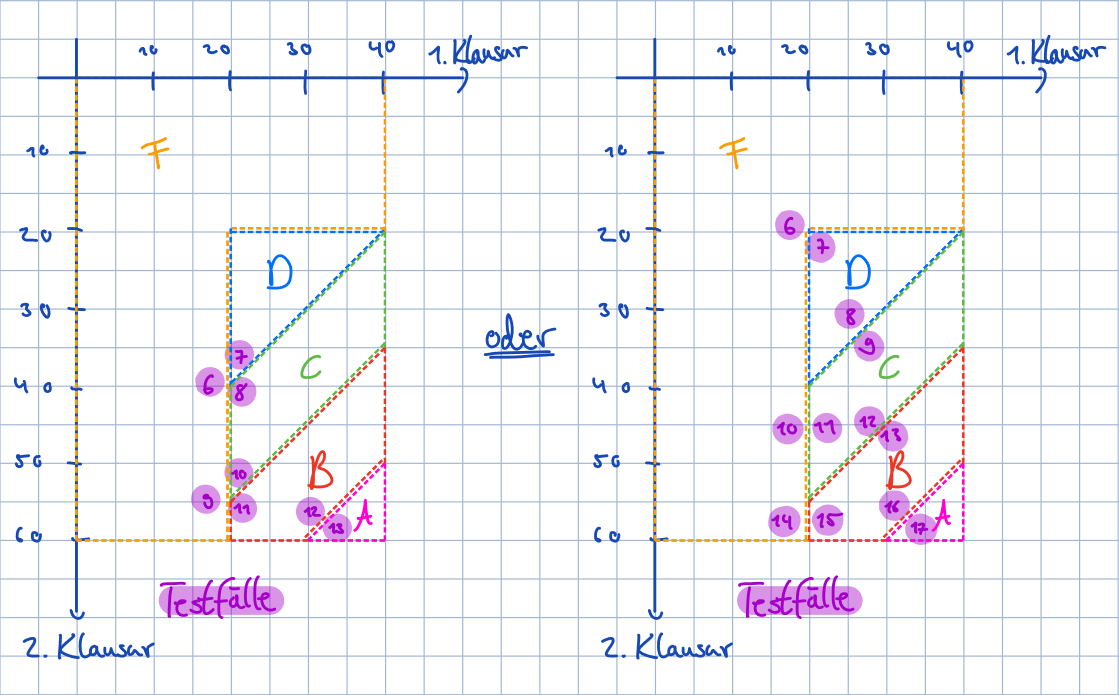
\includegraphics[scale=0.4]{src/u11/garfik.png} 
        \item Wir haben die Testfälle anhand der linke Grafik erstellt.
        \item[] \begin{tabular}{|l|l|l|}
            \hline
            Nr. &  Äquivalenzklasse & Testfall (\& Erwarteter Rückgabewert)\\ \hline  
            6 & Note F & (40,19), Note F\\ \hline 
            7 & Note D & (39,20), Note D\\ \hline 
            8 & Note C & (40,20), Note C\\ \hline 
            9 & Note F & (55,19), Note F\\ \hline 
            10 & Note C & (54,20), Note C\\ \hline 
            11 & Note B & (55,20), Note B\\ \hline 
            12 & Note B & (60,29), Note B\\ \hline 
            13 & Note A & (60,30), Note A\\ \hline 
        \end{tabular}
    \end{itemize}

     % /////////////////////// d) ///////////////////////// 
    \item Installieren Sie die „Eclipse IDE for Java Developers“ (\url{http://www.eclipse.org}) auf Ihrem Computer. Laden Sie sich das vorbereitete Java-Projekt grader-project.zip aus dem KVV herunter und importieren Sie es in Eclipse („Import existing project“ und wählen Sie die ZIP-Datei aus). Die oben beschriebene Funktionalität ist in der Methode Grader.grade(int firstExam, int secondExam) implementiert; sie liegt nur als Bibliothek, nicht aber im Quellcode vor. Implementieren Sie die Testfälle der Aufgaben b) und c) als JUnit-Testfälle in der vorhandenen Testklasse GraderTest.java. Gruppieren Sie Ihre Testfälle sinnvoll in Testmethoden und benennen Sie diese aussagekräftig. Geben Sie Ihre Testklasse mit ab. 
    
    Führen Sie die Testfälle aus: Haben sie Versagen aufgedeckt? Falls ja, stellen Sie mindestens zwei Hypothesen über den/die zu Grunde liegende/n Defekt/e auf. Nehmen Sie die Punkte der untigen Checkliste als Anhaltspunkte: Ihre beiden Hypothesen müssen sich auf zwei verschiedene Punkte beziehen; bitte geben Sie die entsprechenden Punkte mit an.
    
    \begin{itemize}
        \lstinputlisting[language=java, linerange={18}, firstnumber = 18]{src/u11/GraderTest.java}
        
        \item Im Testfall 13 haben wir ein Versagen aufgedeckt. 
        \\ 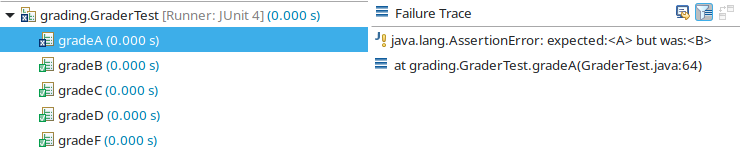
\includegraphics[scale=0.8]{src/u11/output.png} \\
        
        \item Wir vermuten, dass es durch einen falschen Vergleichsoperatoren (Abzweigungen 8.) verursacht wird. 
        \item Oder vielleicht liegt es daran, dass zuerst erst der if Zweig für Note B abgefragt wird und danach der if Zweig für Note A. (Abzweigung: Wurde die Ausführungsreihenfolge von if-else Zweigen beachtet?)
    \end{itemize}
\end{enumerate}

\end{document}